\documentclass[10pt]{article}
\usepackage[utf8]{inputenc}
\usepackage[swedish]{babel}

\def\ordf{Erik Månsson}
\def\sekr{Johan Karlberg}
\def\fvc{Sophia Grimmeiss Grahm}

\def\doctype{Handlingar} %ex. Kallelse, Handlingar, Protkoll
\def\mname{Höstterminsmötet} %ex. styrelsemöte, vårterminsmöte
\def\mnum{HT/17} %ex S02/16, E01/15, VT/13
\def\date{2017-11-14} %YYYY-MM-DD
\def\docauthor{\sekr}

\def\mtime{17:15}
\def\place{E:B}

\usepackage{../../_sektion-handlingar/e-handlingar-sek}
\usepackage{../../e-mote}
\usepackage{../../../../e-sek}

\begin{document}

\firstpage{{\doctype} till {\mname} {\mnum}}{{\date} {\mtime} i {\place}}

\tableofcontents
\newpage

\subfile{../../_sektion-handlingar/_other/guide}
\newpage

\section{Dagordning}
\subsection{Tid och plats}
\tidplats

\subsection{Föredragningslista}
\begin{paralist}
    \pli{TaFMÖ}{}
    \pli{Val av mötesordförande}{}
    \pli{Val av mötessekreterare}{}
    \pli{Godkännande av tid och sätt}{}
    \pli{Val av två justeringspersoner}{}
    \pli{Adjungeringar}{}
    \pli{Godkännande av dagordningen}{}
    \pli{Föregående sektionsmötesprotokoll}{}
    \pli{Meddelanden}{}
    \pli{Beslutsuppföljning}{}
    \pli{Utskottsrapporter}{}
    \pli{Uppföljning av verksamhetsplan}{}
    \pli{Ekonomisk rapport}{}
    \pli{Uttag ur Sektionens fonder sedan förra terminsmötet}{}
    \pli{Resultatrapport från första halvan av verksamhetsåret}{}

    \pli{Behandling av motioner}{}
        \begin{paralist}
          \pli{Döp om Kontaktor till Kommunikator}{}
          \pli{Ändra namnet på likabehandlingsombudet}{}
          \pli{Namnbyte av funktionärspost}{}
          \pli{Veckoliga Studiekvällar med tilltugg}{}
        \end{paralist}
    \pli{Behandling av propositioner}{}
        \begin{paralist}
            \pli{Budgetförslag för 2018}{}
            \pli{Verksamhetsplansförslag för 2018}{}
            \pli{Flytta posten alumniansvarig till ENU}{}
            \pli{Barmästare i E6}{}
            \pli{Omstrukturering av CM}{}
            \pli{Namnbyte av Flickor på Teknis}{}
            \pli{Uppdatering av postbeskrivning i InfU}{}
            \pli{Uppdatering av postbeskrivning i Nöjesutskottet}{}
        \end{paralist}
    \pli{Övrigt}{}
    \pli{TaFMA}{}
\end{paralist}

\begin{signatures}{2}
    \emph{I Sektionens tjänst}
    \signature{\ordf}{Ordförande}
    \signature{\sekr}{Kontaktor}
\end{signatures}

\subfile{../_other/ekonomisk_rapport}
\newpage
\addcontentsline{toc}{subsection}{Balansrapport}
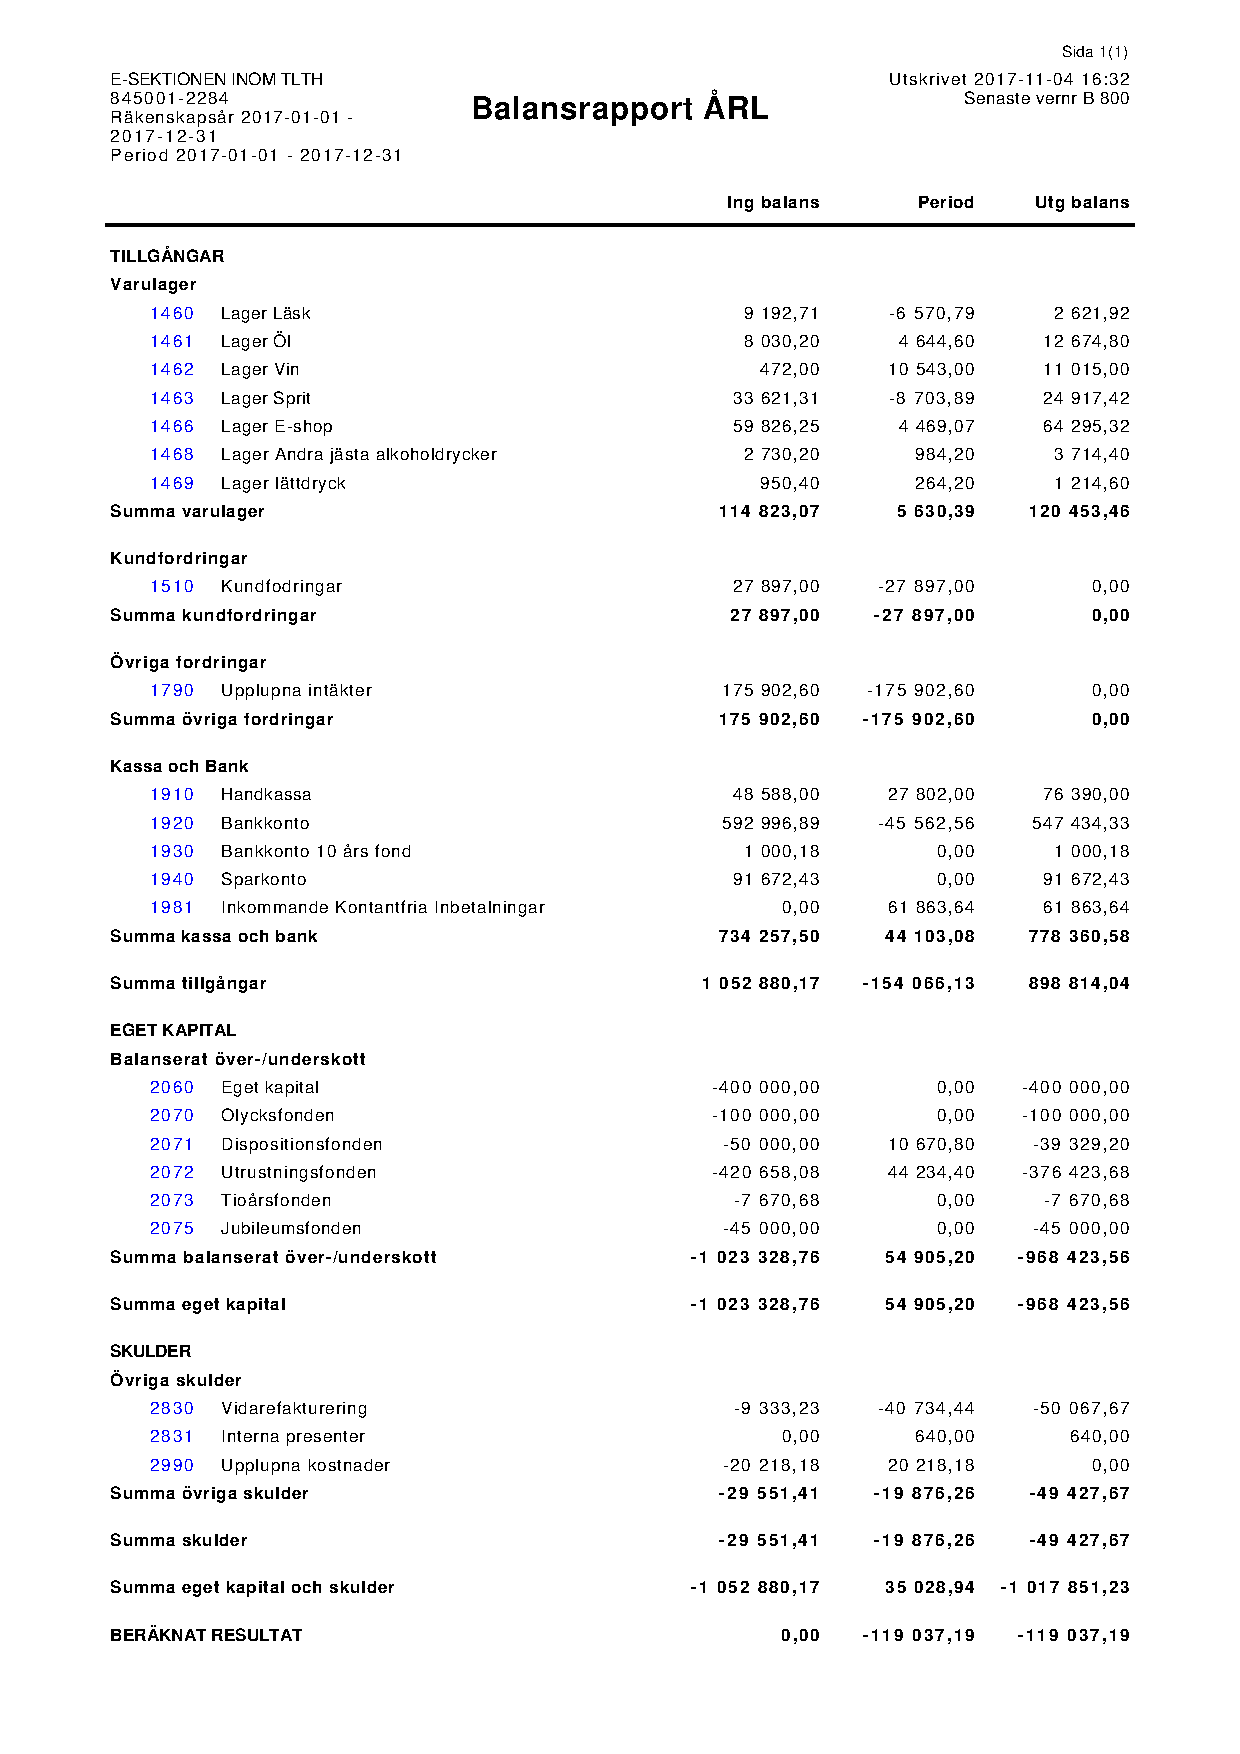
\includepdf[pages=1]{../_res/balansrapport.pdf}

\subfile{../_other/uttag}
\newpage

\begin{supersection}{Beslutsuppföljningar}{}
    \subsection{Överblick}
    \begin{busek}
    \beslutsek{HT/16}{Fanbärare behöver längre påle}{Emil Harvig}{\SI{500}{kr} till inköp av en rundstav, benämnd som påle i vissa sammanhang}{HT/17}

    \beslutsek{HT/16}{Införandet av arbetskläder för utlåning till funktionärer}{Styrelsen 2017}{Sektionen ska tillhandahålla (låna ut) arbetskläder till de behöver det i utskotten}{HT/17}

    \beslutsek{HT/16}{Uppdatering av övervakningspolicyn}{Styrelsen 2017}{Beslut om att att övervakningssystemet ska tas ur bruk tills dess att det uppfyller kraven i övervakningspolicyn}{HT/17}

    \beslutsek{HT/16}{Återremittering av ``Utökning av antal sökande till posten Co-ph{\o}sare''}{Ph{\o}set 16}{}{HT/17}

    \beslutsek{VT/17}{Inköp av banandräkter}{Albin Nyström Eklund}{Elektro Banana Band skulle få en passande utstyrsel i form av banandräkter}{HT/17}

    \beslutsek{VT/17}{Förbättrad förvaring för sektionens lager}{Sanna Nordberg \newline Matilda Dahlström}{Inköp av nya lagerhyllor till CM och Pump för förbättrad förvaring med budget \SI{4000}{kr}}{HT/17}

    \beslutsek{VT/17}{Representations-klädsel åt Inspektorn}{Styrelsen 2017}{Inköp av in en mantel till Inspektorn med budget \SI{2500}{kr}}{HT/17}

    \beslutsek{VT/17}{Äskning av pengar till mentorsprogram}{Erik Månsson, Pontus Landgren}{Äskning av pengar för att utföra mentorsprogrammet}{HT/17}

    \beslutsek{VT/17}{Uppgradering av ljudsystemet i Edekvata}{Styrelsen 2017}{Uppgradering av ljudsystemet i Edekvata med budget \SI{20000}{kr}}{HT/17}

    \beslutsek{VT/17}{Inköp av PA-toppar}{Styrelsen 2017}{En av de två gamla PA-toppar fungerar inte längre}{HT/17}

    \end{busek}

    \newpage
    \subfile{../besuppf/cm-pump}
    \subfile{../besuppf/klader_inspektor}
    \subfile{../besuppf/ljudsystem_edekvata}
    \subfile{../besuppf/mentor}
    \subfile{../besuppf/overvakning}
    \subfile{../besuppf/pa-toppar}
    \subfile{../besuppf/pale}
    \subfile{../besuppf/banan}
    \subfile{../besuppf/arbklader}

\end{supersection}

\begin{utskottsrapporter}
    \subfile{../utskottsrapporter/cm}
    \subfile{../utskottsrapporter/e6}
    \subfile{../utskottsrapporter/enu}
    \subfile{../utskottsrapporter/fvu}
    \subfile{../utskottsrapporter/infu}
    \subfile{../utskottsrapporter/km}
    \subfile{../utskottsrapporter/noju}
    \subfile{../utskottsrapporter/nollu}
    \subfile{../utskottsrapporter/sre}
    \subfile{../utskottsrapporter/styrelsen}
    \subfile{../utskottsrapporter/vb}
\end{utskottsrapporter}

\begin{supersection}{Verksamhetsplaner}{}
   \subfile{../verksplaner/2017}
\end{supersection}

\begin{supersection}{Uppföljningar av verksamhetsplaner}{}
    \subfile{../verksplanuppfar/2017-vt}
    \subfile{../verksplanuppfar/2017-ht}
\end{supersection}

\begin{motioner}
\subfile{../motioner/kontaktor}
\subfile{../motionssvar/kontaktor}
\subfile{../motioner/lika}
\subfile{../motionssvar/lika}
\subfile{../motioner/oumph}
\subfile{../motionssvar/oumph}
\subfile{../motioner/studiek}
\subfile{../motionssvar/studiek}
\end{motioner}

\begin{propositioner}
  \subfile{../propositioner/_budget}
  \subfile{../propositioner/_verkplan}
  \subfile{../propositioner/alumni}
  \subfile{../propositioner/bar}
  \subfile{../propositioner/cm}
  \subfile{../propositioner/fpt}
  \subfile{../propositioner/infu}
  \subfile{../propositioner/noju}
\end{propositioner}

\begin{supersection}{Halvårsbokslut 2017}{}
    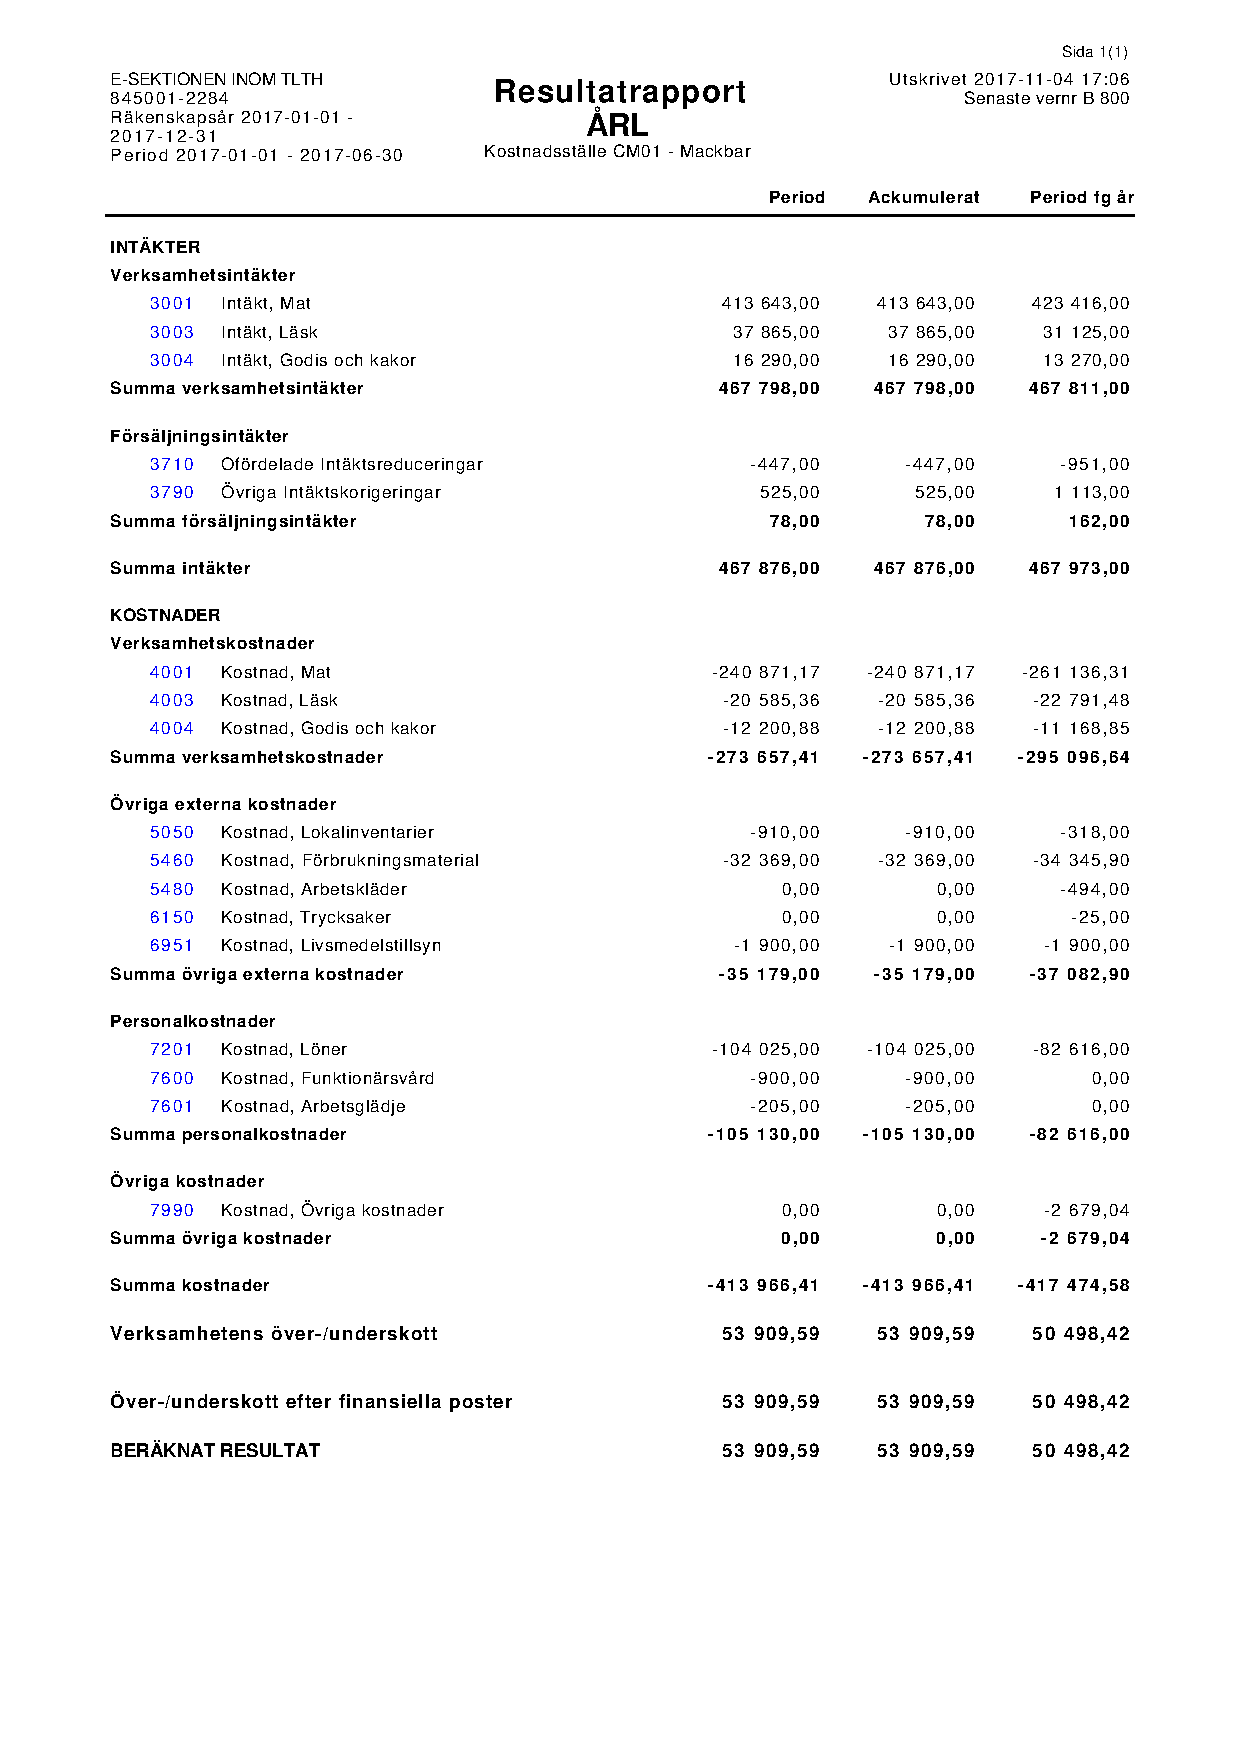
\includepdf[pages=-]{../_res/bokslut/halvarsbokslut.pdf}
\end{supersection}

\end{document}
